\documentclass{note}
%\addtolength{\topmargin}{-2cm}
%\addtolength{\textheight}{2cm}
\usepackage{mathptm,mydef}
\usepackage{courier}
%\renewcommand{\ttdefault}{txtt}
\usepackage[all]{xy}
%\usepackage{MinionPro}

\usepackage{graphicx}
\usepackage{alltt}
\usepackage[T1]{fontenc}
\DeclareGraphicsExtensions{.png,.jpg}

\usepackage{hyperref}
\hypersetup{
    colorlinks, 
    citecolor=black, 
    filecolor=black, 
    linkcolor=blue, 
    urlcolor=black
}

\begin{document}
\small


\begin{center}
 {\large\bf Web Service Standards: Overview}
\end{center}

\vspace*{1cm}

\tableofcontents

\section{Interface Description}
\subsection{WSDL (Web Services Description Language)}
The \bb{WSDL} is an \textcolor{red2}{XML-based IDL}, which is used to describe
the functionality of a web service. 
A WSDL document defines services as collections of network endpoints, or
\bb{ports}. In WSDL, the abstract definition of endpoints and messages is
separated 
from their concrete network deployment or data format bindings. This allows
the reuse of abstract definitions: \bb{messages}, which are abstract
descriptions 
of the data being exchanged, and \bb{port types} which are abstract
collections of 
\bb{operations}. The concrete protocol and data format specifications for a
particular port type constitutes a reusable \bb{binding}. A port is defined by
associating a network address with a reusable binding, and a collection of
ports define a service. Hence, a WSDL document uses the following elements in
the definition of network services: 
\bit
\w \bb{Types}: a container for data type definitions using some type system
(such as XSD); XML schema language (aka XSD) is used for this purpose
\w \bb{Message}: an abstract, typed definition of the data being communicated.
\w \bb{Operation}: an abstract description of an action supported by the
service; SOAP actions and the way the message is encode -- similar to
functino/method call  in PL
\w \bb{Port Type}: an abstract set of operations supported by one or more
endpoints;  {\em defines a web service, the operations that can be performed
  and the messages that are used to perform the operation}
\w \bb{Binding}: a concrete protocol and data format specification for a
particular port type; specifies the interface and defines the SOAP binding
style (RPC/Document) and transport (SOAP protocol); also defines operations
\w \bb{Endpoint (Port in 1.0)}:  a single endpoint defined as a combination of a
binding and a network address. typically represented by a simple \bb{HTTP URL}
string 
\w \bb{Service}: a collection of related endpoints.
\eit


\begin{figure*}[hbt]
\centerline{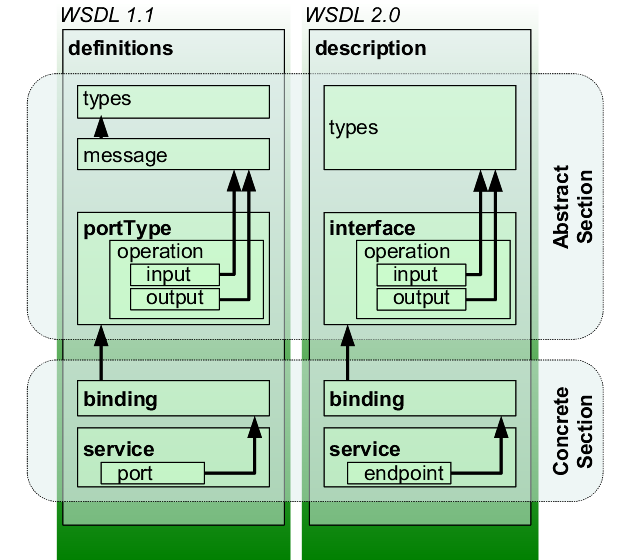
\includegraphics[width=8cm]{pics/wsdl}}
%\centerline{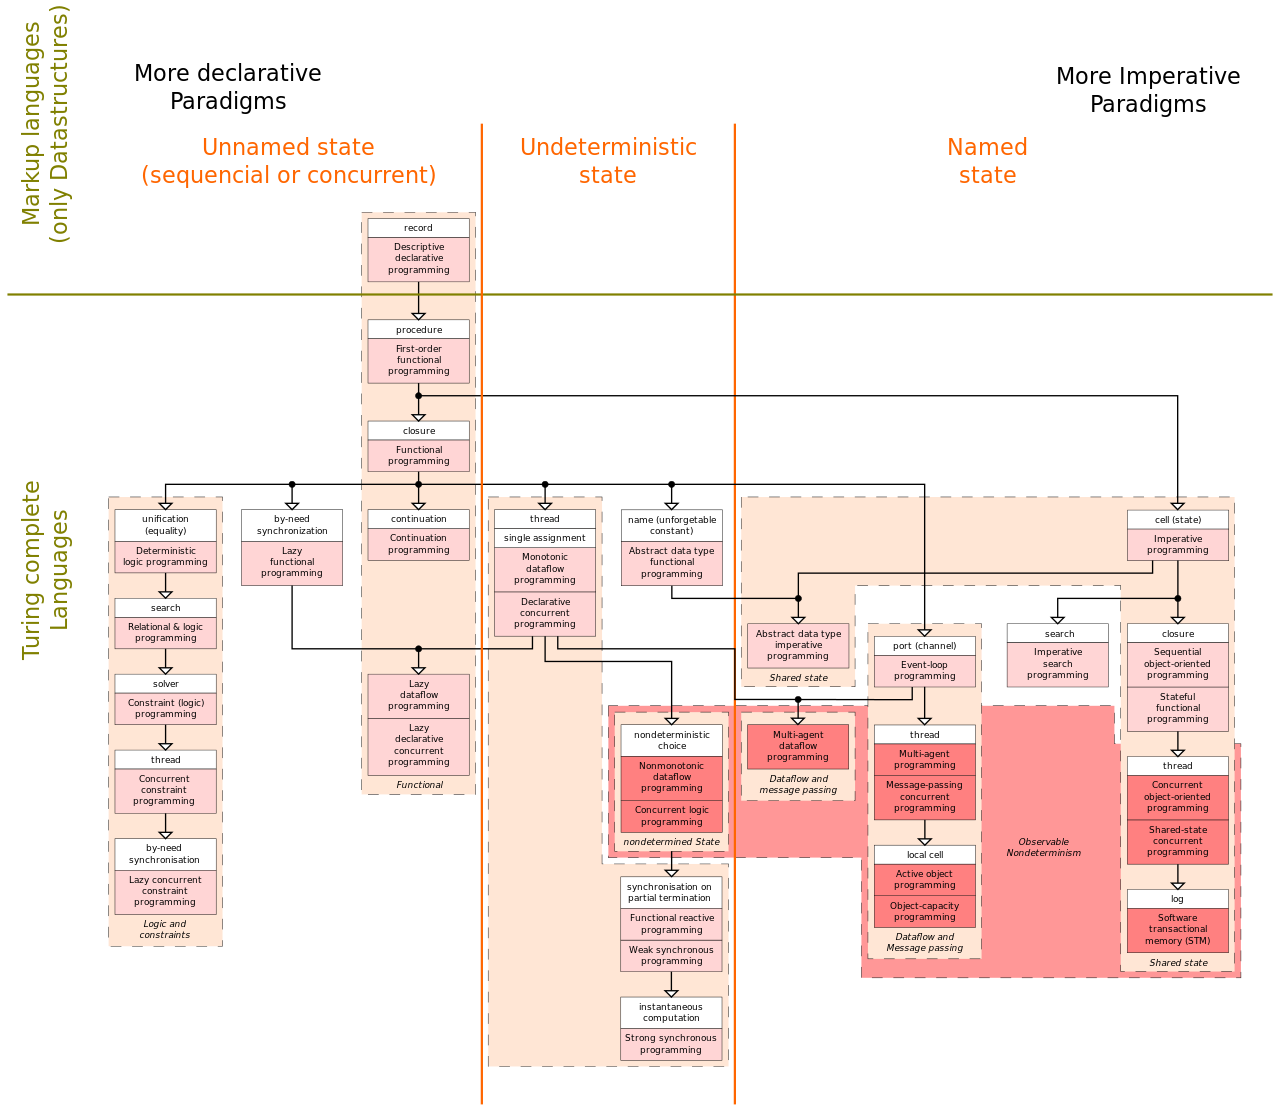
\includegraphics[width=16cm]{prog-paradigms}}
\caption{WSDL 1.0 vs 2.0}
\end{figure*}

\subsubsection{WSDL Document Example}
\begin{alltt}
<?xml version="1.0"?>
<definitions name="StockQuote"

targetNamespace="http://example.com/stockquote.wsdl"
          xmlns:tns="http://example.com/stockquote.wsdl"
          xmlns:xsd1="http://example.com/stockquote.xsd"
          xmlns:soap="http://schemas.xmlsoap.org/wsdl/soap/"
          xmlns="http://schemas.xmlsoap.org/wsdl/">

    <types>
       <schema targetNamespace="http://example.com/stockquote.xsd"
              xmlns="http://www.w3.org/2000/10/XMLSchema">
           <element name="TradePriceRequest">
              <complexType>
                  <all>
                      <element name="tickerSymbol" type="string"/>
                  </all>
              </complexType>
           </element>
           <element name="TradePrice">
              <complexType>
                  <all>
                      <element name="price" type="float"/>
                  </all>
              </complexType>
           </element>
       </schema>
    </types>

    <message name="GetLastTradePriceInput">
        <part name="body" element="xsd1:TradePriceRequest"/>
    </message>

    <message name="GetLastTradePriceOutput">
        <part name="body" element="xsd1:TradePrice"/>
    </message>

    <portType name="StockQuotePortType">
        <operation name="GetLastTradePrice">
           <input message="tns:GetLastTradePriceInput"/>
           <output message="tns:GetLastTradePriceOutput"/>
        </operation>
    </portType>
    <binding name="StockQuoteSoapBinding" type="tns:StockQuotePortType">
        <soap:binding style="document" 
                      transport="http://schemas.xmlsoap.org/soap/http"/>
        <operation name="GetLastTradePrice">
           <soap:operation soapAction="http://example.com/GetLastTradePrice"/>
           <input>
               <soap:body use="literal"/>
           </input>
           <output>
               <soap:body use="literal"/>
           </output>
        </operation>
    </binding>

    <service name="StockQuoteService">
        <documentation>My first service</documentation>
        <port name="StockQuotePort" binding="tns:StockQuoteBinding">
           <soap:address location="http://example.com/stockquote"/>
        </port>
    </service>

</definitions>
\end{alltt}

\section{Service Discovery}

\subsection{UDDI: (Universal Description, Discovery, and Integration)}
UDDI, \textcolor{red2}{\em which is obsolete now\/}, 
provides a systematic way to publish and discover (search) services.
UDDI business registration consists of three components:
\bit
\w \bb{White Pages}: address, contact, and known identifiers;
\w \bb{Yellow Pages}: industrial categorizations based on standard taxonomies
\w \bb{Green Pages}: technical information about services exposed by the
business. 
\eit

\paragraph{White Pages}
White pages give information about the business supplying the service. This
includes the name of the business and a description of the business --
potentially in multiple languages. Using this information, it is possible to
find a service about which some information is already known (for example,
locating a service based on the provider's name). 

Contact information for the business is also provided -- for example the
businesses address and phone number; and other information such as the Dun \&
Bradstreet Universal Numbering System number. 

\paragraph{Yellow Pages}
Yellow pages provide a classification of the service or business, based on
standard taxonomies. These include the Standard Industrial Classification
(SIC), the North American Industry Classification System (NAICS), or the
United Nations Standard Products and Services Code (UNSPSC) and geographic
taxonomies. 

Because a single business may provide a number of services, there may be
several Yellow Pages (each describing a service) associated with one White
Page (giving general information about the business). 

\paragraph{Green Pages}
Green pages are used to describe how to access a Web Service, with information
on the service bindings. Some of the information is related to the Web Service
- such as the address of the service and the parameters, and references to
specifications of interfaces. Other information is not related directly to
the Web Service - this includes e-mail, FTP, CORBA and telephone details for
the service. Because a Web Service may have multiple bindings (as defined in
its WSDL description), a service may have multiple Green Pages, as each
binding will need to be accessed differently. 

\subsection{WS-Discovery (Web Services Dynamic Discovery)}
Web Services Dynamic Discovery (WS-Discovery) is a technical specification
that defines a multicast discovery protocol to locate services on a \textcolor{red2}{local
network}. It operates over TCP and UDP port 3702 and uses IP multicast address 
239.255.255.250. As the name suggests, the actual communication between nodes
is done using web services standards, notably SOAP-over-UDP.  


This specification defines a discovery protocol to locate services. The primary scenario for discovery is a client searching for one or more target services. The protocol defines two modes of operation, an ad hoc mode and a managed mode. In an ad hoc mode, to find a target service by the type of the target service, a scope in which the target service resides, or both, a client sends a probe message to a multicast group; target services that match the probe send a response directly to the client. To locate a target service by name, a client sends a resolution request message to the same multicast group, and again, the target service that matches sends a response directly to the client.

To minimize the need for polling in an ad hoc network, when a target service joins the network, it sends an announcement message to the same multicast group. By listening to this multicast group, clients can detect newly available target services without repeated probing.

To scale to a large number of endpoints and to extend the reach of the
protocol beyond the range of an ad hoc network, this specification defines a
managed mode of operation and a multicast suppression behavior if a discovery
proxy is available on the network. In managed mode, target services send
unicast announcement messages to a discovery proxy and clients send unicast
probe and resolve messages to a discovery proxy. To reduce multicast traffic,
when a discovery proxy detects a probe or resolution request sent multicast on
an ad hoc network, it sends an announcement for itself. By listening for these
announcements, clients detect discovery proxies and switch to a managed mode
of operation and send unicast probe and resolve messages directly to a
discovery proxy. However, if a discovery proxy is unresponsive, clients revert
to an ad hoc mode of operation. 

To support networks with explicit network management services like DHCP, DNS,
domain controllers, directories, etc., this specification acknowledges that
clients and/or target services can be configured to behave differently than
defined herein. For example, another specification may define a well-known
DHCP record containing the address of a discovery proxy, and compliance with
that specification may require client and target services to operate in a
managed mode and send messages to this discovery proxy rather than to a
multicast group. While the specific means of such configuration is beyond the
scope of this specification, it is expected that any such configuration would
allow clients and/or target services to migrate smoothly between
carefully-managed and ad hoc networks. 

\subsubsection{Terms and definitions}
Defined below are the basic definitions for the terms used in this
specification. 
\bit
\w \bb{Target Service}:
An endpoint that makes itself available for discovery.
\w \bb{Client}:
An endpoint that searches for Target Service(s).
\w \bb{Discovery Proxy}:
An endpoint that facilitates discovery of Target Services by Clients.
\w \bb{Hello}:
A message sent by a Target Service when it joins a network; this message
contains key information for the Target Service. A Hello message is also sent
by a Discovery Proxy to reduce multicast traffic on an ad hoc network; this
message contains key information about the Discovery Proxy. 
\w \bb{Bye}:
A best-effort message sent by a Target Service when it leaves a network.
\w \bb{Probe}:
A message sent by a Client searching for a Target Service by Type and/or Scope.
\w \bb{Resolve}:
A message sent by a Client searching for a Target Service by name.
\w \bb{Type}:
An identifier for a set of messages an endpoint sends and/or receives (e.g., a WSDL 1.1 portType, see [WSDL 1.1]).
\w \bb{Scope}:
An extensibility point that allows Target Services to be organized into logical groups.
\w \bb{Metadata}:
Information about the Target Service; includes, but is not limited to,
transports and protocols a Target Service understands, Types it implements,
and Scopes it is in. 
\w \bb{Ad hoc Mode}:
An operational mode of discovery in which the Hello, Bye, Probe and Resolve
messages are sent multicast. 
\w \bb{Managed Mode}:
An operational mode of discovery in which the Hello, Bye, Probe and Resolve
messages are sent unicast to a Discovery Proxy. 
\w \bb{Ad hoc Network}:
A network in which discovery is performed in an ad hoc mode.
\w \bb{Managed Network}:
A network in which discovery is performed in a managed mode.
\eit

\subsubsection{Example Probe sent multicast in ad hoc mode}
\begin{alltt}
<s:Envelope
   xmlns:a="http://www.w3.org/2005/08/addressing"
   xmlns:d="http://docs.oasis-open.org/ws-dd/ns/discovery/2009/01"
   xmlns:i="http://printer.example.org/2003/imaging"
   xmlns:s="http://www.w3.org/2003/05/soap-envelope" >
   <s:Header>
      <a:Action>
         http://docs.oasis-open.org/ws-dd/ns/discovery/2009/01/Probe
      </a:Action>
      <a:MessageID>
         urn:uuid:0a6dc791-2be6-4991-9af1-454778a1917a
      </a:MessageID>
      <a:To>urn:docs-oasis-open-org:ws-dd:ns:discovery:2009:01</a:To>
   </s:Header>
   <s:Body>
      <d:Probe>
         <d:Types>i:PrintBasic</d:Types>
         <d:Scopes
            MatchBy="http://oasis-open.org/ws-dd/ns/discovery/ldap" >
            ldap:///ou=engineering,o=examplecom,c=us
         </d:Scopes>
      </d:Probe>
   </s:Body>
</s:Envelope>
\end{alltt}
\subsubsection{Example ProbeMatch sent in response to Probe}
\begin{alltt}
<s:Envelope
  xmlns:a="http://www.w3.org/2005/08/addressing"
  xmlns:d="http://docs.oasis-open.org/ws-dd/ns/discovery/2009/01"
  xmlns:i="http://printer.example.org/2003/imaging"
  xmlns:s="http://www.w3.org/2003/05/soap-envelope" >
  <s:Header>
    <a:Action>
      http://docs.oasis-open.org/ws-dd/ns/discovery/2009/01/ProbeMatches
    </a:Action>
    <a:MessageID>
      urn:uuid:e32e6863-ea5e-4ee4-997e-69539d1ff2cc
    </a:MessageID>
    <a:RelatesTo>
      urn:uuid:0a6dc791-2be6-4991-9af1-454778a1917a
    </a:RelatesTo>
    <a:To>
    http://www.w3.org/2005/08/addressing/anonymous
    </a:To>
    <d:AppSequence InstanceId="1077004800" MessageNumber="2" />
  </s:Header>
  <s:Body>
    <d:ProbeMatches>
      <d:ProbeMatch>
        <a:EndpointReference>
          <a:Address>
            urn:uuid:98190dc2-0890-4ef8-ac9a-5940995e6119
          </a:Address>
        </a:EndpointReference>
        <d:Types>i:PrintBasic i:PrintAdvanced</d:Types>
        <d:Scopes>
          ldap:///ou=engineering,o=examplecom,c=us
          ldap:///ou=floor1,ou=b42,ou=anytown,o=examplecom,c=us
          http://itdept/imaging/deployment/2004-12-04
        </d:Scopes>
        <d:XAddrs>http://prn-example/PRN42/b42-1668-a</d:XAddrs>
        <d:MetadataVersion>75965</d:MetadataVersion>
      </d:ProbeMatch>
    </d:ProbeMatches>
  </s:Body>
</s:Envelope>
\end{alltt}

\section{Service Activation and Messaging}
\subsection{SOAP (Simple Object Activation Protocol)}
SOAP, originally defined as Simple Object Access Protocol, is a protocol
specification for exchanging structured information in the implementation of
web services in computer networks. It relies on XML Information Set for its
message format, and usually relies on other application layer protocols, most
notably Hypertext Transfer Protocol (HTTP) or Simple Mail Transfer Protocol
(SMTP), for message negotiation and transmission. 

\textcolor{red2}{\em At this point, REST is favored over SOAP in web
  programming. Both uses HTTP for transport but REST is more or less AllJoyn
  CRUD of attribute while SOAP is more like general method invocation. --
  Google-search ``REST vs SOAP'' for details.\/}.  

\begin{alltt}
POST /InStock HTTP/1.1
Host: www.example.org
Content-Type: application/soap+xml; charset=utf-8
Content-Length: 299
SOAPAction: "http://www.w3.org/2003/05/soap-envelope"
 
<?xml version="1.0"?>
<soap:Envelope xmlns:soap="http://www.w3.org/2003/05/soap-envelope">
  <soap:Header>
  </soap:Header>
  <soap:Body>
    <m:GetStockPrice xmlns:m="http://www.example.org/stock">
      <m:StockName>IBM</m:StockName>
    </m:GetStockPrice>
  </soap:Body>
</soap:Envelope>
\end{alltt}

\section{Service Orchestration}
\subsection{WS-BPEL (Business Process Execution Language)}
\subsubsection{History}
\bit
\w IBM had ``programming in the large'' language \textcolor{red2}{\bf{}WSFL} (Web Services Flow
Language)
\w Microsoft had its own ``programming in the large'' language
\textcolor{red2}{\bf{}XLANG} 
\bit
\w \bb{programming in the large}\footnote{``By large programs we mean systems consisting of many small programs
  (modules), possibly written by different people. We need languages for
  programming-in-the-small, i.e. languages not unlike the common programming
  languages of today, for writing modules. We also need a {\em module
  interconnection language\/} for knitting those modules together into an
  integrated whole and for providing an overview that formally records the
  intent of the programmer(s) and that can be checked for consistency by a
  compiler. We explore the software reliability aspects of such an
  interconnection language. Emphasis is placed on facilities for information
  hiding and for defining layers of virtual machines''}: e.g. module
interconnection language, Meadowview
  \eit

\w \textcolor{red2}{\bf{}BPML} (Business Process Modeling Language) was proposed
popular 
\w Later, \textcolor{red2}{\bf{}BPEL} (a.k.a. WS-BPEL, BPEL4WS) became the de
facto standard. 
\eit

\subsubsection{Orchestration vs Choreography}
   \bit
   \w \textcolor{blue2}{BPEL is an {\bf{}orchestration} language, not a {\bf
    choreography} language}. 
   \w \bb{orchestration}: \underline{executable} process that involves message exchanges
   with other systems, such that the message exchange sequences
   (i.e. \textcolor{red2}{\bf{}''protocol''}) are controlled by the
   orchestration designer

   \w \bb{choreography}: specifies a protocol for peer-to-per interactions,
   defining, e.g. the legal sequences of messages exchanged with the purpose
   of guaranteeing interoperability
        \bit
        \w more of a ``specification'' than ``programming''
        \w consider CCS, CSP, $\pi$-calculus
        \w \bb{NOT executable}
        \w \textcolor{red2}{ONE GOAL of MEADOWVIEW: Make an {\em executable\/}
          choreography language} 
        \eit
   \eit

\subsubsection{Example purchaseOrderProcess}
\textcolor{red2}{\em The following are ``un-XML-ized'' version.}

\begin{alltt}
   // IDL -- WSDL definition
   message \textbf{POMessage} \{
     customerInfoType customerInfo;
     purchaseOrderType purchaseOrder;
   \};
   message \textbf{InvMessage} \{
     InvoiceType IVC;
   \};
   message \textbf{orderFaultType} \{
     OrderFault problemInfo;
   \};

   message \textbf{shippingRequestMessage} \{
     customerInfo info;
   \};
   message \textbf{shippingInfoMessage} \{
     shippingInfo info;
   \};
   message \textbf{scheduleMessage} \{
     scheduleInfo schedule
   \};
\end{alltt}

\begin{alltt}
  // Ports: supported by purchase order process
  // non-first-class version of SV interface
  port \textbf{purchaseOrderPort} \{
    operation \textbf{sendPurchseOrder}(input POMessage po;
                               output InvMessage inv;
                               fault orderFaultType failure);
  \};
  port \textbf{invoiceCallbackPort} \{
    operation \textbf{sendInvoice}(input InvMessage inv);
  \};
  port \textbf{shippingCallbackPort} \{
    operation \textbf{sendSchedule}(input scheduleMessage msg);
  \};  
\end{alltt}

\begin{alltt}
  // Ports: supported by shipping services
  port \textbf{shippingPort} \{
    operation \textbf{requestShipping}(input shippingRequestMessage msg,
                              output shippingInfoMessage msg,
                              fault orderFaultType failure);
  \};
\end{alltt}

\begin{alltt}
  // Ports: supported by invoice services
  port \textbf{computePricePort} \{
    operation \textbf{initiatePriceCalculation}(input POMessage msg);
    operation \textbf{sendShippingPrice}(input shippingInfoMessage msg);
  \};
\end{alltt}

\begin{alltt}
  // Ports: supported by production scheduling process
  port \textbf{schedulingPort} \{
    operation \textbf{requestProductionScheduling}(input POMessage msg);
    operation \textbf{sendShippingSchedule}(input scheduleMessage msg);
  \};
\end{alltt}

Let $P_0$ and $P_1$ be processes, where $P_i$ already defines its services
using WSDL (IDL).  ``Links'' are used to model relationships between partner
processes -- e.g. between $P_0$ and $P_1$.

\begin{alltt}
  // Link -- Partner Links
  link \textbf{purchasingLink} \{
    // role <role-type> <role-name>
    role purchaseOrderPort purchaseService;
  \};
  link \textbf{invoicingLink} \{
    role computePricePort invoiceService;
  \};
  link \textbf{shippingLink} \{
    role shippingPort shippingService;
    role shippingCallbackPort shippingRequester;
  \};
  link \textbf{schedulingLink} \{
    role schedulingPort schedulingService;
  \};
\end{alltt}

\begin{alltt}
  // PROCESS
  process \textbf{purchaseOrderProcess} \{
    // partner links
    puchasingLink purchasing(purchasingService /*myrole*/);
    invoicingLink invoicing(invoiceRequester /*myrole*/,
                            invoiceService /*partnerrole*/);
    shippingLink shipping(shippingRequester /*myrole*/,
                          shippingSerivce /*partnerrole*/);
    schedulingLink scheduling(schedulingService /*partnerrole*/);

    // variables
    POMessage PO;
    InvMessage Invoice;
    shippingRequestMessage shippingRequest;
    shippingInfoMessage shippingInfo;
    scheduleMessage shippingSchedule;

    // fault handlers
    faultHandler \{
      catch (cannotCompleteOrder(POFaultType POFault)) \{
        reply(purchasing /*link*/, 
      \};
    \};

    sequence \{
      receive(purchasing /*link - shippingPort*/, 
              sendPurchaseOrder /*operation*/, PO /*bound*/);

      // arrows
      arrow ship-to-invoice;
      arrow ship-to-scheduling;

      // sequence #1: CENTER
      sequence \{
        $shippingRequest.customerInfo = $PO.customerInfo;

        // decide on shipper
        invoke(shipping /*link - shippingPort*/, 
               \textbf{requestShipping} /*operation*/,
               shippingRequest /*input*/,
               shippingInfo /*output */,
               source=ship-to-invoice /* arrow */);

        // arrange logistics
        receive(shipping /*link - shippingCallbackPort*/,  
                sendSchedule /*operation*/, shippingSchedule /*bound*/,
                source=ship-to-scheduling /*arrow*/);
      \};

      // sequence #2: LEFT (INVOICE)
      sequence \{
        // initial price calculation
        invoke(invoicing /*link - computePricePort */, 
               \textbf{initiatePriceCalculation} /*operation*/,
               PO /*input*/);

        // complete price calculation
        invoke(invoicing /*link - computePricePort */, 
               \textbf{sendShippingPrice} /*operation*/,
               shippingInfo /*input*/,
               target=ship-to-invoice /*arrow*/);

        receive(invoicing /*link - invoiceCallbackPort*/,  
                \textbf{sendInvoice} /*operation*/, Invoice);
      \};      

      // sequence #3: RIGHT (SHIPPING)
      sequence \{
         ...        
      \};      
    \};
  \};
\end{alltt}

\section{Service Choreography}
\subsection{WS-CDL (Web Services Choreography Description Language)}
\subsubsection{WS-CDL model overview}
WS-CDL describes interoperable, peer-to-peer collaborations between
participants. In order to facilitate these collaborations, services commit to
mutual responsibilities by establishing formal relationships. Their
collaboration takes place in a jointly agreed set of ordering and constraint
rules, whereby information is exchanged between the participants. 

The WS-CDL model consists of the following entities:
\bit
\w \bb{roleType, relationshipType and participantType}: Within a choreography,
information is always exchanged between participants within or across trust
boundaries. All interactions occur between roles being exhibited by
participants, and are constrained by a relationship. Within WS-CDL, a
participant is abstractly modeled by a participantType, a role by a roleType,
and a relationship by a relationshipType:
    \bit
    \w A \bb{participantType} groups together those parts of the observable behavior that must be implemented by the same logical entity or abstract organization
    \w A \bb{roleType} enumerates potential observable behavior a participantType can exhibit in order to interact
    \w A \bb{relationshipType} identifies the mutual commitments that must be
    made 
    for collaborations to be successful
    \eit

\w \bb{informationType, variable and token}: A variable contains information
about commonly observable objects in a collaboration, such as the information
exchanged or the observable information of the roleTypes involved. A token is
an alias that can be used to reference parts of a variable. Information
exchange variables, state capturing variables and tokens have informationTypes
that define the type of information the variable contains or the token
references 

\w \bb{choreography}: A choreography defines collaborations between
interacting participantTypes:
     \bit
     \w \bb{choreography life-line}: The choreography life-line expresses the
     progression of a collaboration. Initially, the collaboration is
     established between participants, then work is performed within it and
     finally it completes either normally or abnormally 
     \w \bb{choreography exception blocks}: An exception block specifies what
     additional actions should occur when a choreography behaves in an
     abnormal way 
     \w \bb{choreography finalizer blocks}: A finalizer block specifies
     additional actions that should occur to modify the effect of an earlier
     successfully completed choreography, for example to confirm or undo the
     effect 
     \eit
\w \bb{channelType}: A channel realizes a point of collaboration between
participantTypes by specifying where and how information is exchanged. Within
WS-CDL, channels are abstractly modeled as channelTypes 

\w \bb{workunit}: A workunit prescribes the constraints that must be fulfilled
for making progress, and thus performing work, within a choreography 

\w \bb{activities and ordering structures}: Activities describe the actions
performed within a choreography. Ordering structures combine activities with
other ordering structures in a nested structure to express the ordering rules
of actions performed within a choreography 

\w \bb{interaction activity}: An interaction is the basic building block of a
choreography. It results in an exchange of information between participants
and possible synchronization of their observable information changes 

\w \bb{semantics}: Semantics allow the creation of descriptions that can
record the semantic definitions of every component in the model
\eit

\subsubsection{Interactions}
\bit
\w An \bb{interaction} is the realization of a collaboration between roles.
\w {Roles} are grouped into participants.
\eit
\begin{alltt}
<interaction name="QuoteElicitation" 
             operation="getQuote" 
             channelVariable="tns:Buyer2SellerC">
    <description type="documentation">
        Quote Elicitation
    </description>
    <participate relationshipType="tns:Buyer2Seller" 
                 fromRoleTypeRef="tns:BuyerRole" 
                 toRoleTypeRef="tns:SellerRole"/>
    <exchange name="QuoteRequest" 
              informationType="tns:QuoteRequestType" 
              action="request">
        <description> Quote Request Message Exchange </description>
        <send variable="cdl:getVariable('quoteRequest','','')"/>
        <receive variable="cdl:getVariable('quoteRequest','','')"/>
    </exchange>

    <exchange name="QuoteResponse" 
              informationType="tns:QuoteResponseType" 
              action="respond">
        <description> Quote Response Message Exchange </description>
        <send variable="cdl:getVariable('quoteResponse','','')"/>
        <receive variable="cdl:getVariable('quoteResponse','','')"/>
    </exchange>

    <exchange name="QuoteResponseFault" 
              informationType="tns:QuoteResponseFaultType" 
              action="respond" 
              faultName="InvalidProductFault">
        <description> Quote Response Fault Exchange </description>
        <send variable="cdl:getVariable('faultResponse','','')"/>
        <receive variable="cdl:getVariable('faultResponse','','')"/>
    </exchange>
</interaction>
\end{alltt}

\subsubsection{Roles}
\begin{alltt}
<roleType name="BuyerRole">
    <description> Role for Buyer </description>
    <behavior name="BuyerBehavior" interface="BuyerBehaviorInterface">
        <description> Behavior for Buyer Role </description>
    </behavior>
</roleType>
<roleType name="SellerRole">
    <description> Role for Seller </description>
    <behavior name="SellerBehavior" interface="SellerBehaviorInterface">
        <description> Behavior for Seller </description>
    </behavior>
</roleType>
\end{alltt}

\subsubsection{Participant}
\begin{alltt}
<participantType name="Seller">
     <description> Seller Participant </description>
    <roleType typeRef="tns:SellerRole"/>
</participantType>
<participantType name="Buyer">
    <description> Buyer Participant </description>
    <roleType typeRef="tns:BuyerRole"/>
</participantType>
\end{alltt}

\subsubsection{Relationships}
\begin{alltt}
<relationshipType name="Buyer2Seller">
    <description> Buyer Seller Relationship </description>
    <roleType typeRef="tns:BuyerRole"/>
    <roleType typeRef="tns:SellerRole"/>
</relationshipType>
\end{alltt}


\subsubsection{Workunits}
\begin{alltt}
  Workunit (G) (R) (B is False)
    Body
 ==
  (G) Body (R G) Body (R G) Body
\end{alltt}
\bit
\w In general, it's same as:
\begin{verbatim}
  while (G) 
     Body
  until (!R)
\end{verbatim}
\w If G is true, 
\begin{verbatim}
  repeat
    Body
  until (!R)
\end{verbatim}
\w If R is false, 
\begin{verbatim}
  If (G)
    Body
\end{verbatim}
\eit

\begin{alltt}
  Boolean barteringDone@Seller = false
  Elicit a quote from the seller
  repeat \{ 
    choice \{
      \{
        Accept the quote and place the order
        barteringDone@Seller = true
      \}
      \{
        Reject the quote and ask for a new quote
      \}
     \}
  \} until (barteringDone@Seller == false) 
\end{alltt}

\subsubsection{Choices}

\subsection{WSCI (Web Service Choreography Interface)}
\subsection{WSCL (Web Service Conversation Language)}


\end{document}
